% Auto-generated on 2026-04-08 from results/version_a tables
% Source files: table2_main_results.csv, table3_hard_test_calibration.csv, spearman_table.csv

\begin{table}[t]
\centering
\caption{Main results on ETHICS virtue (Qwen2.5-0.5B).}
\label{tab:main-results-version-a}
\begin{tabular}{lcc}
\toprule
Condition & Test Acc. (\%) & 95\% CI (\%) \\
\midrule
Baseline (empty prefix) & 20.20 & [19.10, 21.31] \\
Neutral prefix (best L) & 20.18 & [19.07, 21.31] \\
Instruction-only paraphrase (best K->k) & 62.28 & [61.56, 63.01] \\
GRPO best & 37.46 & [36.78, 38.13] \\
\bottomrule
\end{tabular}
\end{table}

\begin{table}[t]
\centering
\caption{Hard-test accuracy and calibration (ETHICS virtue, Qwen2.5-0.5B).}
\label{tab:hard-calibration-version-a}
\begin{tabular}{lcc}
\toprule
Condition & Hard Acc. (\%) & ECE \\
\midrule
Baseline & 20.23 & 0.4975 \\
GRPO best & 37.50 & 0.3741 \\
\bottomrule
\end{tabular}
\end{table}

\begin{table}[t]
\centering
\caption{Spearman correlation between $\Delta L_{dev}(L)$ and test accuracy across all $(L, K\to k, seed)$ tuples.}
\label{tab:spearman-version-a}
\begin{tabular}{lcc}
\toprule
Task/Model & Spearman $\rho$ & 95\% CI \\
\midrule
Virtue / Qwen2.5-0.5B & 0.7253 & [0.4556, 0.8660] \\
\bottomrule
\end{tabular}
\end{table}

\begin{figure}[t]
\centering
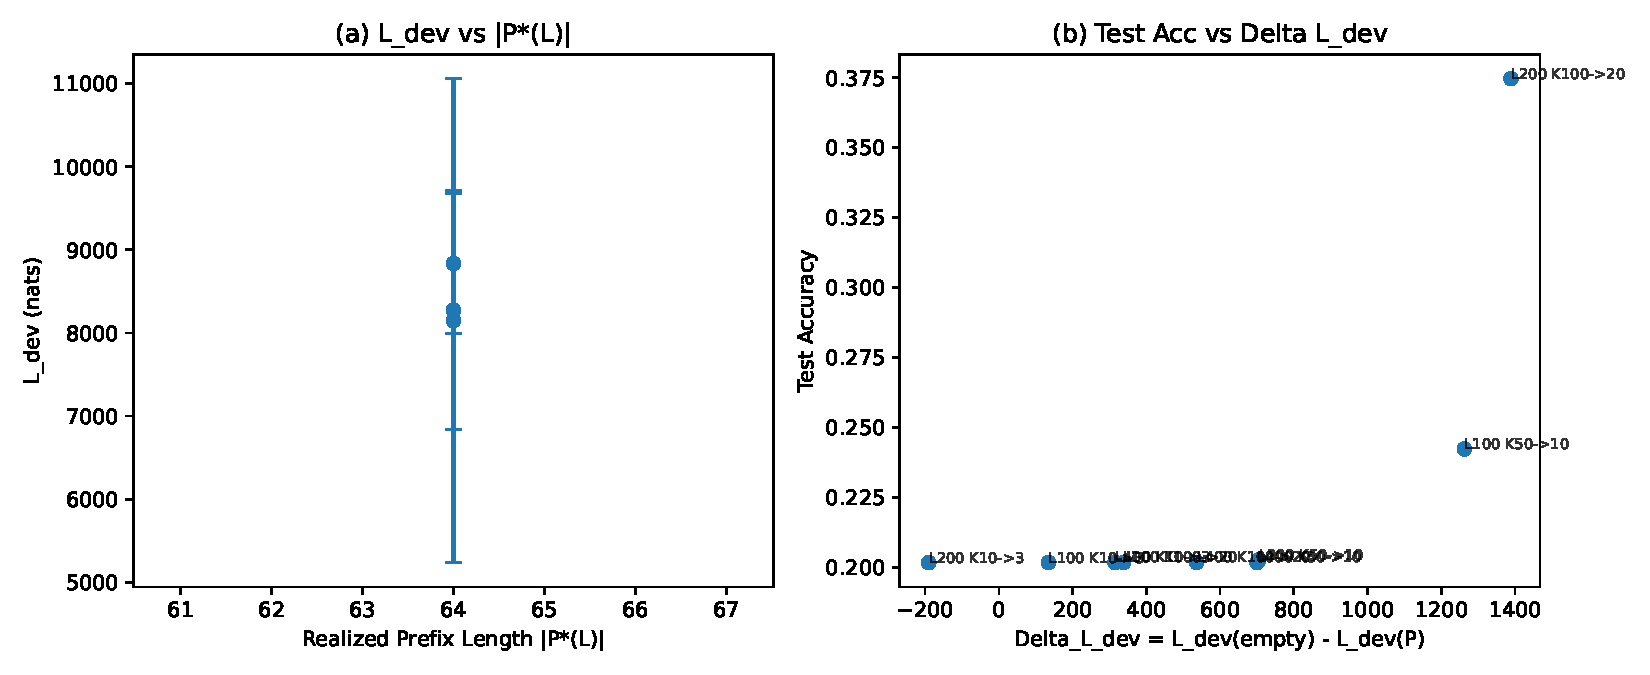
\includegraphics[width=0.95\linewidth]{results/version_a/figures/mdl_curves.pdf}
\caption{MDL proxy curves for ETHICS virtue (Qwen2.5-0.5B): (a) $L_{dev}(P^*(L))$ vs. prefix length and (b) test accuracy vs. $\Delta L_{dev}(L)$.}
\label{fig:mdl-curves-version-a}
\end{figure}

% Note: split hashes and reproducibility metadata are documented in:
% results/version_a/reproducibility_note_2026-04-08.md
